\section{Preliminaries}
\label{main_preliminaries}
In this section, we provide the problem definition for our CortexDebate, and introduce the McKinsey Trust Formula which plays an important role in our proposed CortexDebate.

\subsection{Problem Definition}
\label{problem_definition}

Our CortexDebate establishes a directed debating graph among $n$ LLM agents, $\mathcal{G}=(\mathcal{A}, \mathcal{E})$, where $\mathcal{A}=\left \{A_{i} \right \} _{i=1}^{n} $ is the vertex set representing participating LLM agents and $\mathcal{E}=\left \{E_{i\to j} \right \}_{i,j\in \left [1,2,...,n  \right ] }$ is the directed edge set representing information transmission. Here, each directed edge $E_{i\to j}$ is assigned a weight $W_{i\to j}$ that indicates the expected improvement in the performance of agent $A_{j}$ by debating with $A_{i}$. All the weights $\left \{ W_{i\to j}  \right \}$ are dynamically optimized during the debate process. Given a problem $Q$, the agents $\left \{ A_{i}  \right \}_{i=1}^{n}$ engage in $D$ rounds of debate. In the $d$-th debate round, each LLM agent $A_{i}$ scrutinizes the outputs of the LLM agents connected to it, and then generates its own output $O_{i}^{d}$ along with a self-confidence score $H_{i}^{d}$. Afterwards, the final answer of this debate round, $\textit{i.e.}$, $F_{d}$, is obtained by majority voting.


\begin{figure*}[t]
\centering
  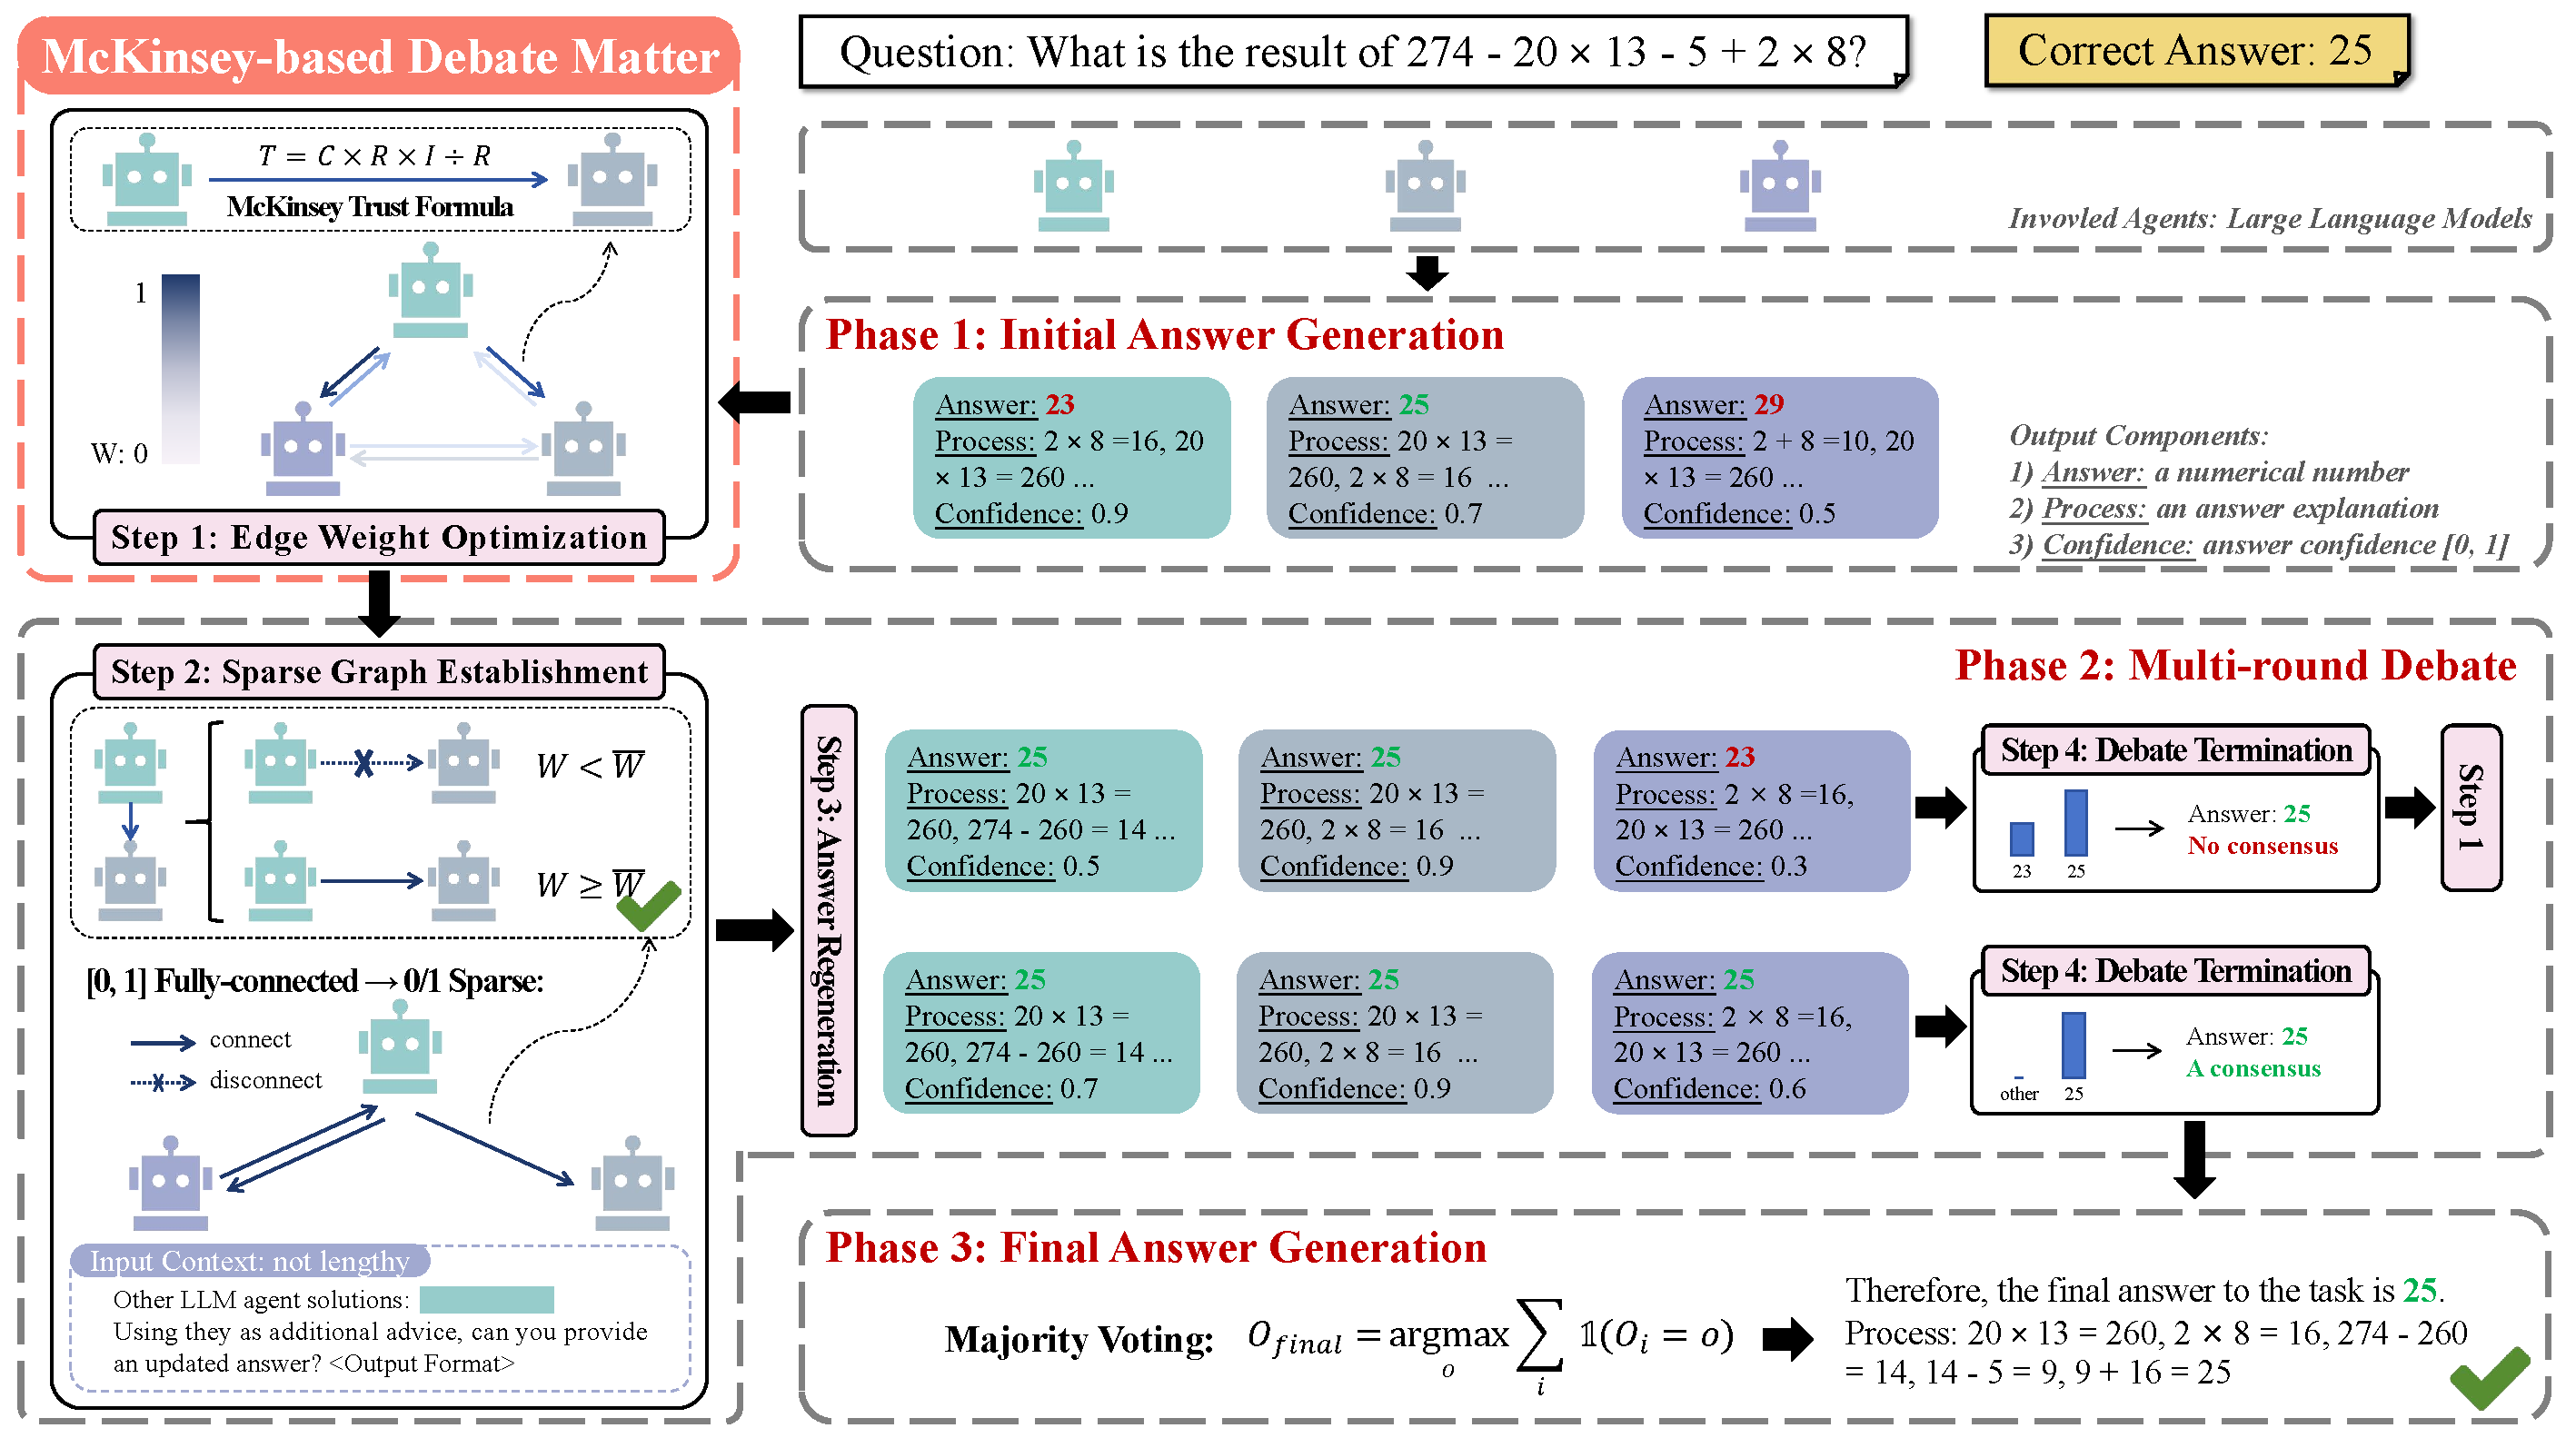
\includegraphics[width=\linewidth]{pic/method_simple.pdf}
  \caption {Overview of our proposed CortexDebate, which is inspired by the working mode of human brain cortex and consists of three phases: (a) Initial Answer Generation: Each LLM agent generates an answer, an explanation, and its confidence score. (b) Multi-round Debate: Participating LLM agents engage in debates guided by a sparse debating graph which is dynamically optimized by MDM module. (c) Final Answer Generation: After multi-round debates, the final answer is generated by majority voting.}
  \label{cortex}
\end{figure*}


\subsection{McKinsey Trust Formula}
\label{mckinsey_trust_formula}

The McKinsey Trust Formula~\citep{lamarre2012mckinsey} is widely used in sociology to evaluate the level of trustworthiness of a person within a group. This formula can be expressed as:
\begin{equation}
\setlength{\abovedisplayskip}{1mm}
\setlength{\belowdisplayskip}{1mm}
  \label{MTF}
  T= \frac{C\times R\times I}{S},
\end{equation}
\noindent where $C$, $R$, $I$, and $S$ denote credibility, reliability, intimacy, and self-orientation, respectively. Among them, credibility measures professional competence, reliability measures the stability of task performance, intimacy measures the relationship with the evaluated person, and self-orientation measures the self-orientation level of the evaluated person within a group.

In our MDM module, we adapt these four factors to the context of MAD. Specifically, for directed edge $E_{i\to j}$ connecting agent $A_{i}$ to $A_{j}$, credibility evaluates the professional competence of $A_{i}$. Reliability is the average confidence score of $A_{i}$ to its own answers in history debates, which represents the performance reliability on the current question. Intimacy represents the average degree of difference in viewpoints between $A_{i}$ and $A_{j}$ in history debates, as the collision of different viewpoints can enhance the debating effectiveness~\cite{xiong2023examining}. Self-orientation represents the participation level of $A_{i}$ in the debate (a lower participation level indicates higher self-orientation).